\chapter{Privacy Filters}
\label{cha:privacy-filters}
As discussed in section \ref{sec:problem-context}, the goal of this chapter is to find a solution to the information leakage problems that exist within Solid. This problem arises due to the fact no distinction is made between the trust level given to client applications. These applications either get the full resource or nothing, but since mostly structured data is handled by Solid, it should be possible to restrict which parts of a resource are exposed.

As illustrated by figure \ref{fig:privacy-utility-tradeoff}, improved privacy always comes with a trade-off regarding data utility. Evidently, data with less or less precise attribute values will be more private, but this same property also renders the data less useful. Making this trade-off is very context-dependent (how much is the application trusted, what kind of data is requested etc.). As such, rendering data more private must happen dynamically, at the time of a request, such that details of the request can be taken into account when determining what kind of transformations ought to happen to the data.

\begin{figure}[h]
    \centering
    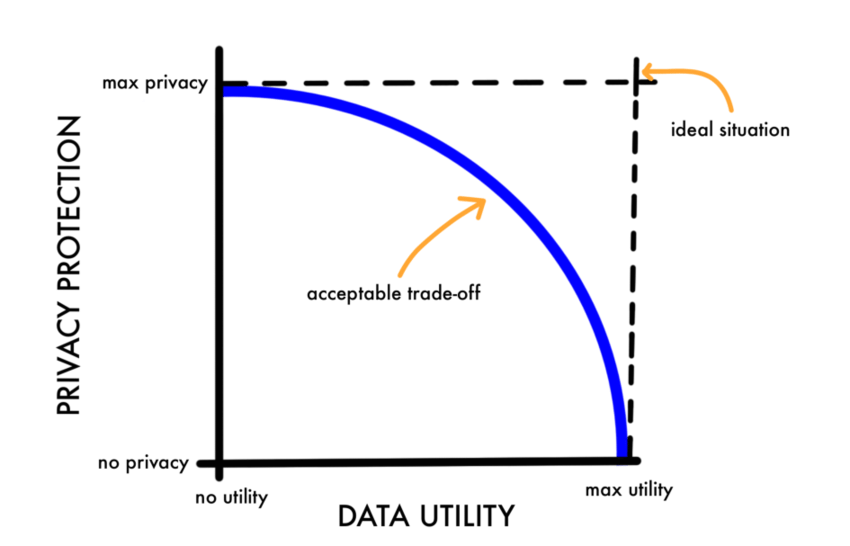
\includegraphics[width=0.8\textwidth]{images/Data-Privacy-Protection-versus-Data-Utility.png}
    \caption{Illustration of the privacy-utility trade-off, from \citet{datasharing-implications}}
    \label{fig:privacy-utility-tradeoff}
\end{figure}

\noindent This chapter introduces the concept of \textit{privacy filters}, which dynamically strip away attributes of exposed data in accordance with some predefined rules. A prototype that implements privacy filters is developed for the \gls{CSS}: \middleware{} (short for Privacy-enhancing Plugin for Solid Applications). \middleware{} provides a middleware in the Solid server which provides more fine-grained privacy control options. 

In the developed prototype privacy filters are represented by a JSON document (per data scheme), describing which transformations ought to happen to which data attribute. Users can then specify how much privacy they want (in general, or for specific datatypes). When a request is received, \middleware{} checks what data type it is and what level of privacy the user has requested. Subsequently, a number of transformations are applied to the data (as specified by the privacy filter configuration file), after which the transformed data is returned to the application. An example of what such a rewrite can look like is provided in figure \ref{fig:example-treatment-privacy-filter}.

The next sections discusses how \middleware{} was designed by listing the requirements that were envisioned before its development, followed by a detailed description of the subsequent design decisions and implementation details. Evaluation of the developed prototype is discussed in chapter \ref{cha:evaluation}.

\section{Design}
\subsection{Adversary model}
\label{sec:attacker-model}
The attacker model considered in the design and development of \middleware{} handles the case of untrusted applications. In this case, the adversary is thus a Solid application to which the user grants access. Concretely, this means that the application can access any data to which the \gls{ACL}s give it access, and in the modes determined herein. However, there is no fine-grained privacy control, i.e., on the level of a single resource. Consequently, the attacker here is an honest-but-curious attacker, which does not deviate from the Solid protocol and does not attempt to break the access control mechanisms.

It is important to note the goal of \middleware{} in terms of disclosure prevention here. As explained in section \ref{sec:statistical-privacy}, many \gls{PETs} try to prevent identity disclosure (in datasets containing data from many different users). However, since every Solid pod is linked to a WebID (containing data of a single user), the main goal of this middleware is to prevent attribute disclosure. Accordingly, the attackers considered in the two adversary models try to gain knowledge of \textit{data attributes}. Handling identity disclosure is also an important aspect of a privacy-aware software system, but in the case of Solid, this must be handled by data aggregators and other clients collecting data over multiple pods.

\subsection{Requirements}
%\label{sec:requirements}

\subsubsection{Functional requirements}
\textbf{Decentralization} Since \middleware{} builds forth upon the Solid project, it is crucial that it follows the same philosophy. A core property of Solid is its decentralization, implying that anyone can run a Solid server and host their pod themselves. This means that any user can easily set-up \middleware{}. Two options are possible here, either an extension of an existing Solid server, or building a proxy which handles the anonymization aspects and forwards requests to a separate Solid server.\\

\noindent \textbf{Flexibility for the supported data scheme} Solid builds further upon the principles of Linked Data, and Solid servers can store nearly any type of data. As \middleware{} aims to be a general solution, it should work with any type of structured data, i.e., it must provide a way to anonymize \textit{any} type of textually represented structured data. Thus, flexibility for the supported data scheme is an essential part of \middleware{}. Concretely, \middleware{} should not hard-code any supported data schemes nor which PET should be applied to them: these should be able to be plugged in flexibly and selected automatically, to ensure that any data scheme can be supported. This provides a technical challenge, as a sufficient level of abstraction must be developed to be able to support any data scheme, while ensuring that the leakage requirements are not violated. \\

\noindent \textbf{Automatically select \gls{PETs}} Different client applications may be trusted differently, just as that different data schemes may contain more or less sensitive data elements. An important aspect to solve is thus being able to distinguish different \textit{privacy levels}: required levels of anonymization. \middleware{} must therefore not only be able to adapt to different data schemes, but must also support different privacy levels for every data scheme. The selected PET is highly dependent on the data scheme and required level of privacy, therefore \middleware{} must automatically select \gls{PETs} based on the input data scheme and requested privacy level. \\

\noindent \textbf{Extensibility} Finally, the Solid project is still very much a work in progress. This implies that the specification will likely be modified many times in the future, and additional features will be added. If \middleware{} wants to successfully keep interacting with Solid servers, the architecture should be ready to easily be extended in order to support newly released features and modifications. 

\subsubsection{Non-functional requirements}
\textbf{Intuitive to use} Solid aims to become the de-facto standard for web applications in the future. Consequently, it must be intuitive for non-technical users to use this technology. There can be no technical jargon, and it must be incredibly easy to set-up. Since \middleware{} aims to follow this philosophy, the proposed solution must be intuitive to use for non-technical users. 

Concretely, this means that it should be opaque to the users which concrete PET is applied for which use case. On that account, a number of \textit{privacy levels} should be created and presented to the user in a simple manner: a higher privacy level means more data protection but less utility. The user will then be able to select between a number of privacy levels, without needing to understand the technical details behind the scenes. Examples of concrete transformations can be given, to make the effects of selecting a certain level more comprehensible. Section \ref{sec:privacylevels} introduces four privacy levels that are used in the developed proof-of-concept, but these serve only as a concrete example. \\

\noindent \textbf{Testability} Since \middleware{} operates so dynamically, there is a lot of opportunity for bugs to sneak in that will go unnoticed. Some bugs may only appear under the presence of a specific combination of transformations in the configuration files. Therefore, testability is an important aspect. Increased testability gives stronger guarantees of the correct behavior of \middleware{}, which is essential in the context of a privacy-enhancing technology.  

\subsection{Privacy levels}
\label{sec:privacylevels}
\noindent In order to provide an intuitive mechanism for selecting which data is transformed, the concept of privacy levels is introduced. Privacy levels form an abstraction above the concrete data transformations and \gls{PETs} that are applied to the data before it is passed on to the application. This ensures that non-technical users can use a privacy-enhancing middleware, without needing to understand the technical details of the technologies and tactics that are employed. 

\middleware{} is configured with a default privacy level, but also supports specific privacy levels for certain data schemes. For example, a user could configure \middleware{} to use privacy level 2 by default, but privacy level 4 on bank transactions, since he does not want to expose this data. This makes the middleware more context-sensitive and allows for strong configurability. The privacy-utility trade-off can then also be taken into account for specific applications that need data with very high utility to deliver usable results. For every data scheme, an explanation should also be included which specifies concretely what will happen to the data under a certain privacy level.

Another important aspect is that the developers of privacy filters for specific data schemes must be aware of what privacy levels map to what leakage or tactics. This is best determined by privacy experts as it is a very complex topic. However, appendix \ref{appendix:privacy-levels} shows an example of such a mapping that was used to guide the development of configuration files for the prototype of \middleware{}.

\section{Implementation}

\middleware{} is implemented as an extension of the \acrlong{CSS}. The complete code and instructions can be found at \url{https://github.com/jessegeens/pepsa-component}.

\subsection{Design decisions}
In every architectural design, important decisions have to be made based on some sort of cost-benefit analysis: there is no free lunch. Similarly, this is the case with the design of \middleware{}. This section describes the reasoning behind a number of important design decisions that have been made during the modelling and development.

\subsubsection{Positioning}
A first important aspect of the design of \middleware{} is where it is logically positioned. There are two main possibilities, both with their own advantages. 

One possibility would be to make \middleware{} an extension of an existing Solid Server (such as, in our case, the \gls{CSS}). This would result in significantly sped up development, as well as much better performance. A disadvantage of this approach is that it leads to more centralization: if a user is using a pod provided by a third-party not running \middleware{}, there is no way to enable this. Extending an existing solid server also means choosing one specific server to support, making the solution incompatible with other servers.

The other possibility for realising the goals and requirements that were laid out, would be to build \middleware{} as a proxy. Requests from the Solid application would be directed to \middleware{} instead, which fetches the data, sanitizes it, and then replies with the sanitized data. This is a much less centralized option, but comes at a big performance cost. There are is more network usage and double the number of HTTP requests, for example. However, there is also a very important technical limitation. As was discussed in section \ref{sec:solid-oidc}, Solid uses \gls{DPoP} tokens. As can be seen in listing \ref{listing:dpop}, the \texttt{htu} parameter of the \gls{DPoP} token body prevents this token from being used in another pod, essentially making the proxy solution impossible when communicating with a Solid server using this authentication mechanism.

As such, the first option (extending an existing Solid server) is seen as the only possible choice. It also has the additional advantage of fulfilling another requirement. Since this is an extension of the Solid server and does not really interact with the Solid protocol itself, this extension is much easier to keep up-to-date with the quickly evolving Solid specification.

\subsubsection{Supporting multiple data schemes}
Solid supports storing nearly any type of resource, both linked and non-linked. The data that is prone to leakage and that will be most likely requested by applications is structured data. Unstructured data may also contain \gls{PII}, but this is discussed in section \ref{sec:limitations}. Structured data can take many forms, and any good middleware should be independent of the types of structured data that are requested or passing through it. However, \middleware{} needs to perform operations on the data that passes through it, and should thus have some context as to how it should handle a specific data scheme. Two possibilities for tackling this problem were envisioned.

A first possibility would be to have separate components, where each component is responsible for performing transformations on the input data of a specific data scheme. The components would be loaded dynamically at run-time, using dependency injection technology such as \textit{components.js}\footnote{\url{https://componentsjs.readthedocs.io/en/latest/}}. This would result in great flexibility: the transformation component can perform virtually any transformation. However, the big downside of this strategy is that it results in a significant development time for each component (and thus, for every supported data scheme). This can result in a lack of support for many (popular) data schemes, making \middleware{} significantly less useful. Another major downside is that this imposes new weaknesses from a security point-of-view, as untrusted code is imported in and executed on the Solid server.

A second option that was considered was to provide \middleware{} with an internal library of "transformation components", for each content representation. For example, there would be a component that performs pseudonymization on data that is represented in JSON. At startup, the software would then read a number of \textit{scheme configuration files}, one for every supported data scheme. These files then specify how a data scheme should be detected, and what transformations ought to be applied to it. This requires more up-front coding to support this library of transformations for content representations. There is also a computational cost associated with having to parse all these configuration files and apply the rules expressed in them, instead of directly executing code.
Despite these drawbacks, there is also a very large advantage to this approach: supporting new data schemes becomes a much easier and faster task. The only work that needs to be performed to support a new data scheme would be to write a scheme configuration file, something that can be done in a few hundred lines of JSON.

In the end, the second option was opted for. The reason for this is that the cost of writing new components specifically for one data scheme is too high for the relatively meager advantages it gives over the other approach. The appendix contains the JSON Schema used to describe such configuration files (see listing \ref{listing:privacy-filter-jsonschema}) as well as an example of such a scheme configuration file, specifically aimed at use case \ref{usecase:personal-finance} modifying financial data (see listing \ref{listing:privacy-filter-kbc}).

\subsubsection{Supported transformations}
Table \ref{table:supported-transformations} gives an overview of which transformations are currently supported in \middleware{}. The choice for supported transformations is mostly based on the discussion from section \ref{sec:transformation-approaches}. This section discussed a taxonomy of architectural tactics involving data transformations. Some tactics could not be mapped to an equivalent tactic in our middleware because the middleware works on a per-request basis. An example of this is the \textit{Select / Filter} tactic, which keeps a copy of the original data. The \textit{Aggregate} tactic was not applicable as \middleware{} does not support grouping data elements, as data is treated on a per-attribute basis. Similar arguments hold for other tactics that are not supported. The \textit{Perturbation} tactic is based on the \textit{Blur} tactic from table \ref{table:de-id-taxonomy}, but renamed to convey its applicability to numeric values. Similarly, \textit{Encrypt} is supported along with the similar \textit{Hash} tactic.

\begin{table}[H]
\begin{center}
\begin{tabulary}{\textwidth}{p{0.20\textwidth}p{0.8\textwidth}}
\textbf{Transformation name} & \textbf{Description}                                                                                                                                                          \\ \hline
Remove               & The targeted and deliberate omission of PII from the data record or data set.                                                                                                 \\
Pseudonym            & The systematic replacement of direct identifiers with surrogates, whereby the mapping between surrogate and identity is kept separately.                                      \\
Perturbation         & The insertion of randomized noise into the values of the data to hide exact values                                                                                 \\
Random               & Tactics that involve the modification of PII attribute values/records by injecting artificial random elements.                                                                \\
Encrypt              & Using cryptographic means to encode the PII attribute values / records / datasets.                                                                                            \\
Hash                 & Using cryptographic hash functions to obfuscate the PII attribute values / records / datasets in a deterministic fashion.                                                                                            \\
\end{tabulary}
\caption{Overview of data transformations supported in \middleware{}}
\label{table:supported-transformations}
\end{center}
\end{table}

\subsection{Implementation in CSS}
The implementation of \middleware{} is realised as an extension of the \acrlong{CSS}\footnote{\url{https://github.com/solid/community-server}}, leveraging components.js to substitute a component of the \gls{CSS} with a component provided by \middleware{}. An overview of the architecture of the \gls{CSS} is presented in figure \ref{fig:solid-arch}.

Concretely, the main component of \middleware{} is the \texttt{AnonymizingHTTPHandler}, which extends the \texttt{OperationHttpHandler} class provided by the \gls{CSS}. Using a custom components.js configuration, this new class is injected into the \gls{CSS} by giving it as an argument to the \texttt{ParsingHttpHandler}. On diagram \ref{fig:solid-arch}, this is located under \texttt{AuthenticatedLdpHandler}.

A configuration file for the \gls{CSS} specifying the dependency injection of the \texttt{AnonymizingHTTPHandler} can be found in the appendix, under listing \ref{listing:css-config}.

Figure \ref{fig:arch-overview} gives an overview of the system architecture of \middleware{}. Components that are part of a vanilla version of the \gls{CSS} are colored in blue. The red component, \texttt{AnonymizingHTTPHandler}, is the main component of the middleware and is the component that is injected into the \gls{CSS}. The yellow components are also included dynamically through the configuration file (listing \ref{listing:css-config}), such that other content representations can also easily be supported. The \texttt{ParserSelector} can then, based on the content representation that is defined in the detected data scheme, select the correct parser to perform the execution of all specified transformations. 
Figure \ref{fig:pepsa-sequence} illustrates the flow of how a privacy filter is applied to an incoming request in the \gls{CSS}.

\begin{figure}[h]
    \centering
    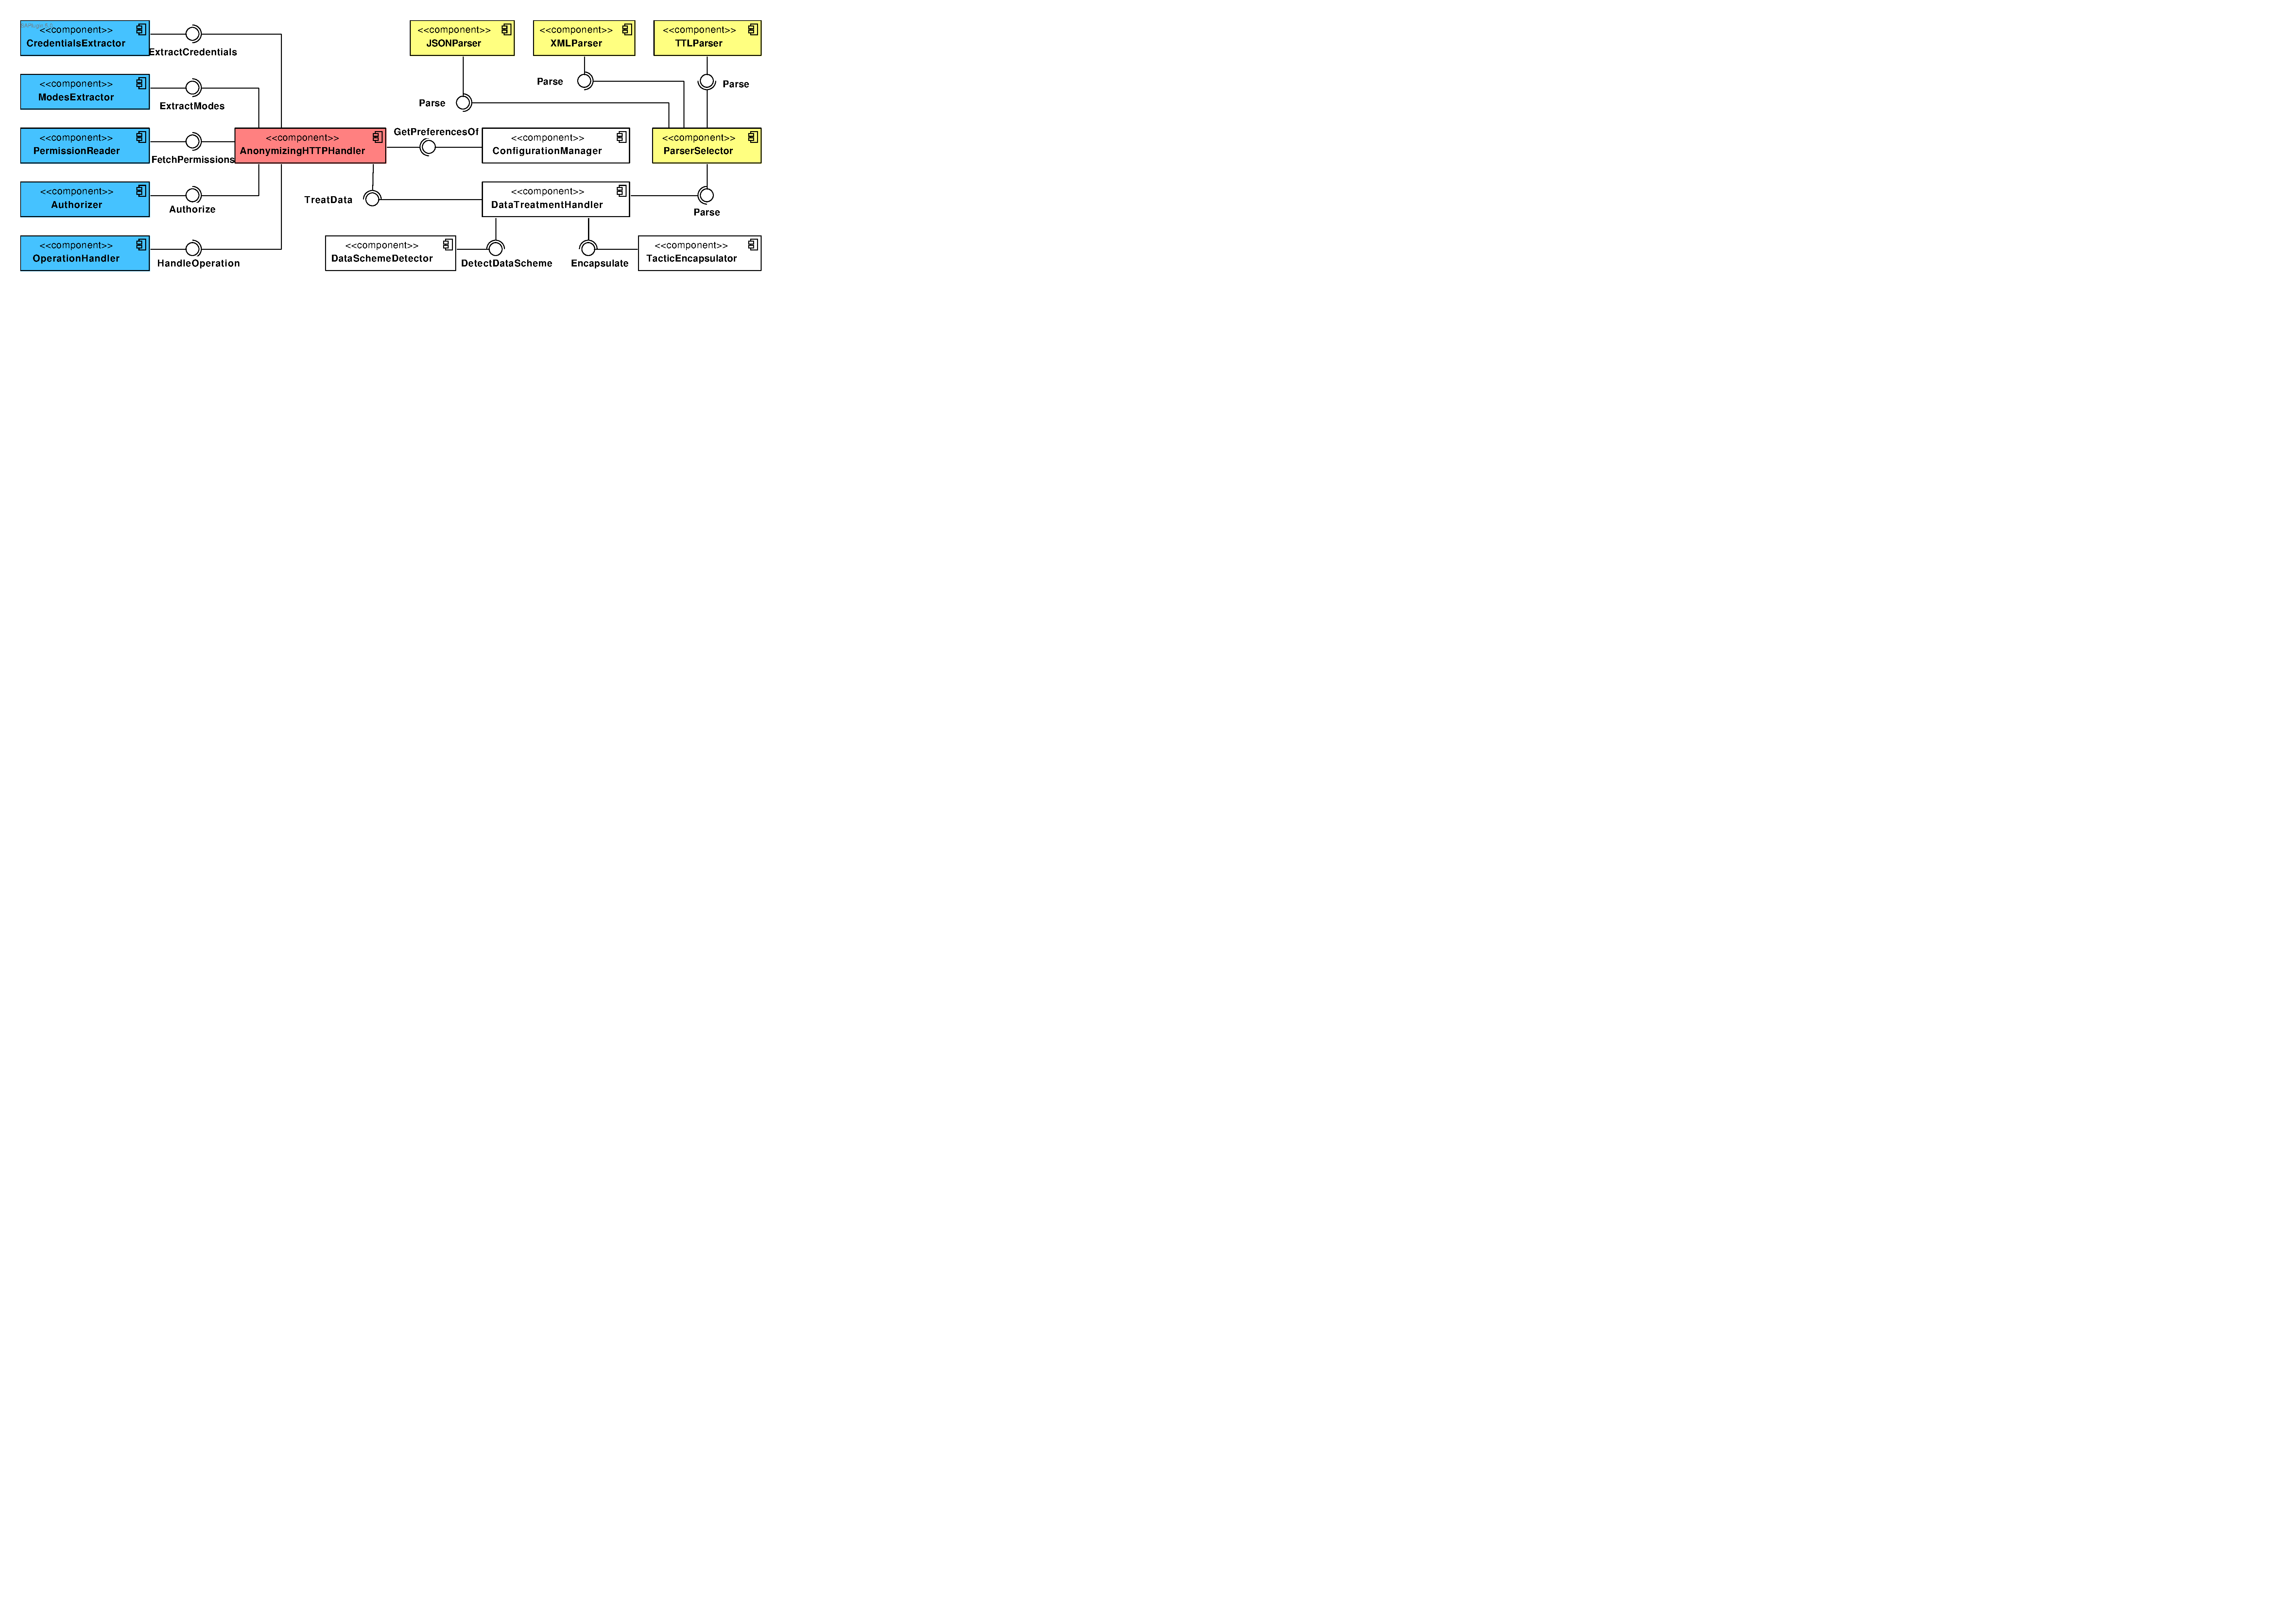
\includegraphics[width=1.0\textwidth]{images/architecture/PePSA-System-Overview.pdf}
    \caption{Overview of \middleware{} architecture}
    \label{fig:arch-overview}
\end{figure}

\todo[inline]{TODO: add example transformed data}
\begin{figure}[h]
\centering
\begin{subfigure}{.5\textwidth}
  \centering
  \begin{minted}[linenos,tabsize=2,breaklines]{json}
  {
  }
  \end{minted}
  \caption{Data before applying privacy filter}
  \label{fig:data-before-privacy-filter}
\end{subfigure}%
\begin{subfigure}{.5\textwidth}
  \centering
  \begin{minted}[linenos,tabsize=2,breaklines]{json}
  {
  }
  \end{minted}
  \caption{Data after applying privacy filter}
  \label{fig:data-after-privacy-filter}
\end{subfigure}
\caption{Example of data treatment by privacy filter, applied to financial transactions data}
\label{fig:example-treatment-privacy-filter}
\end{figure}

\begin{sidewaysfigure}[h]
    \centering
    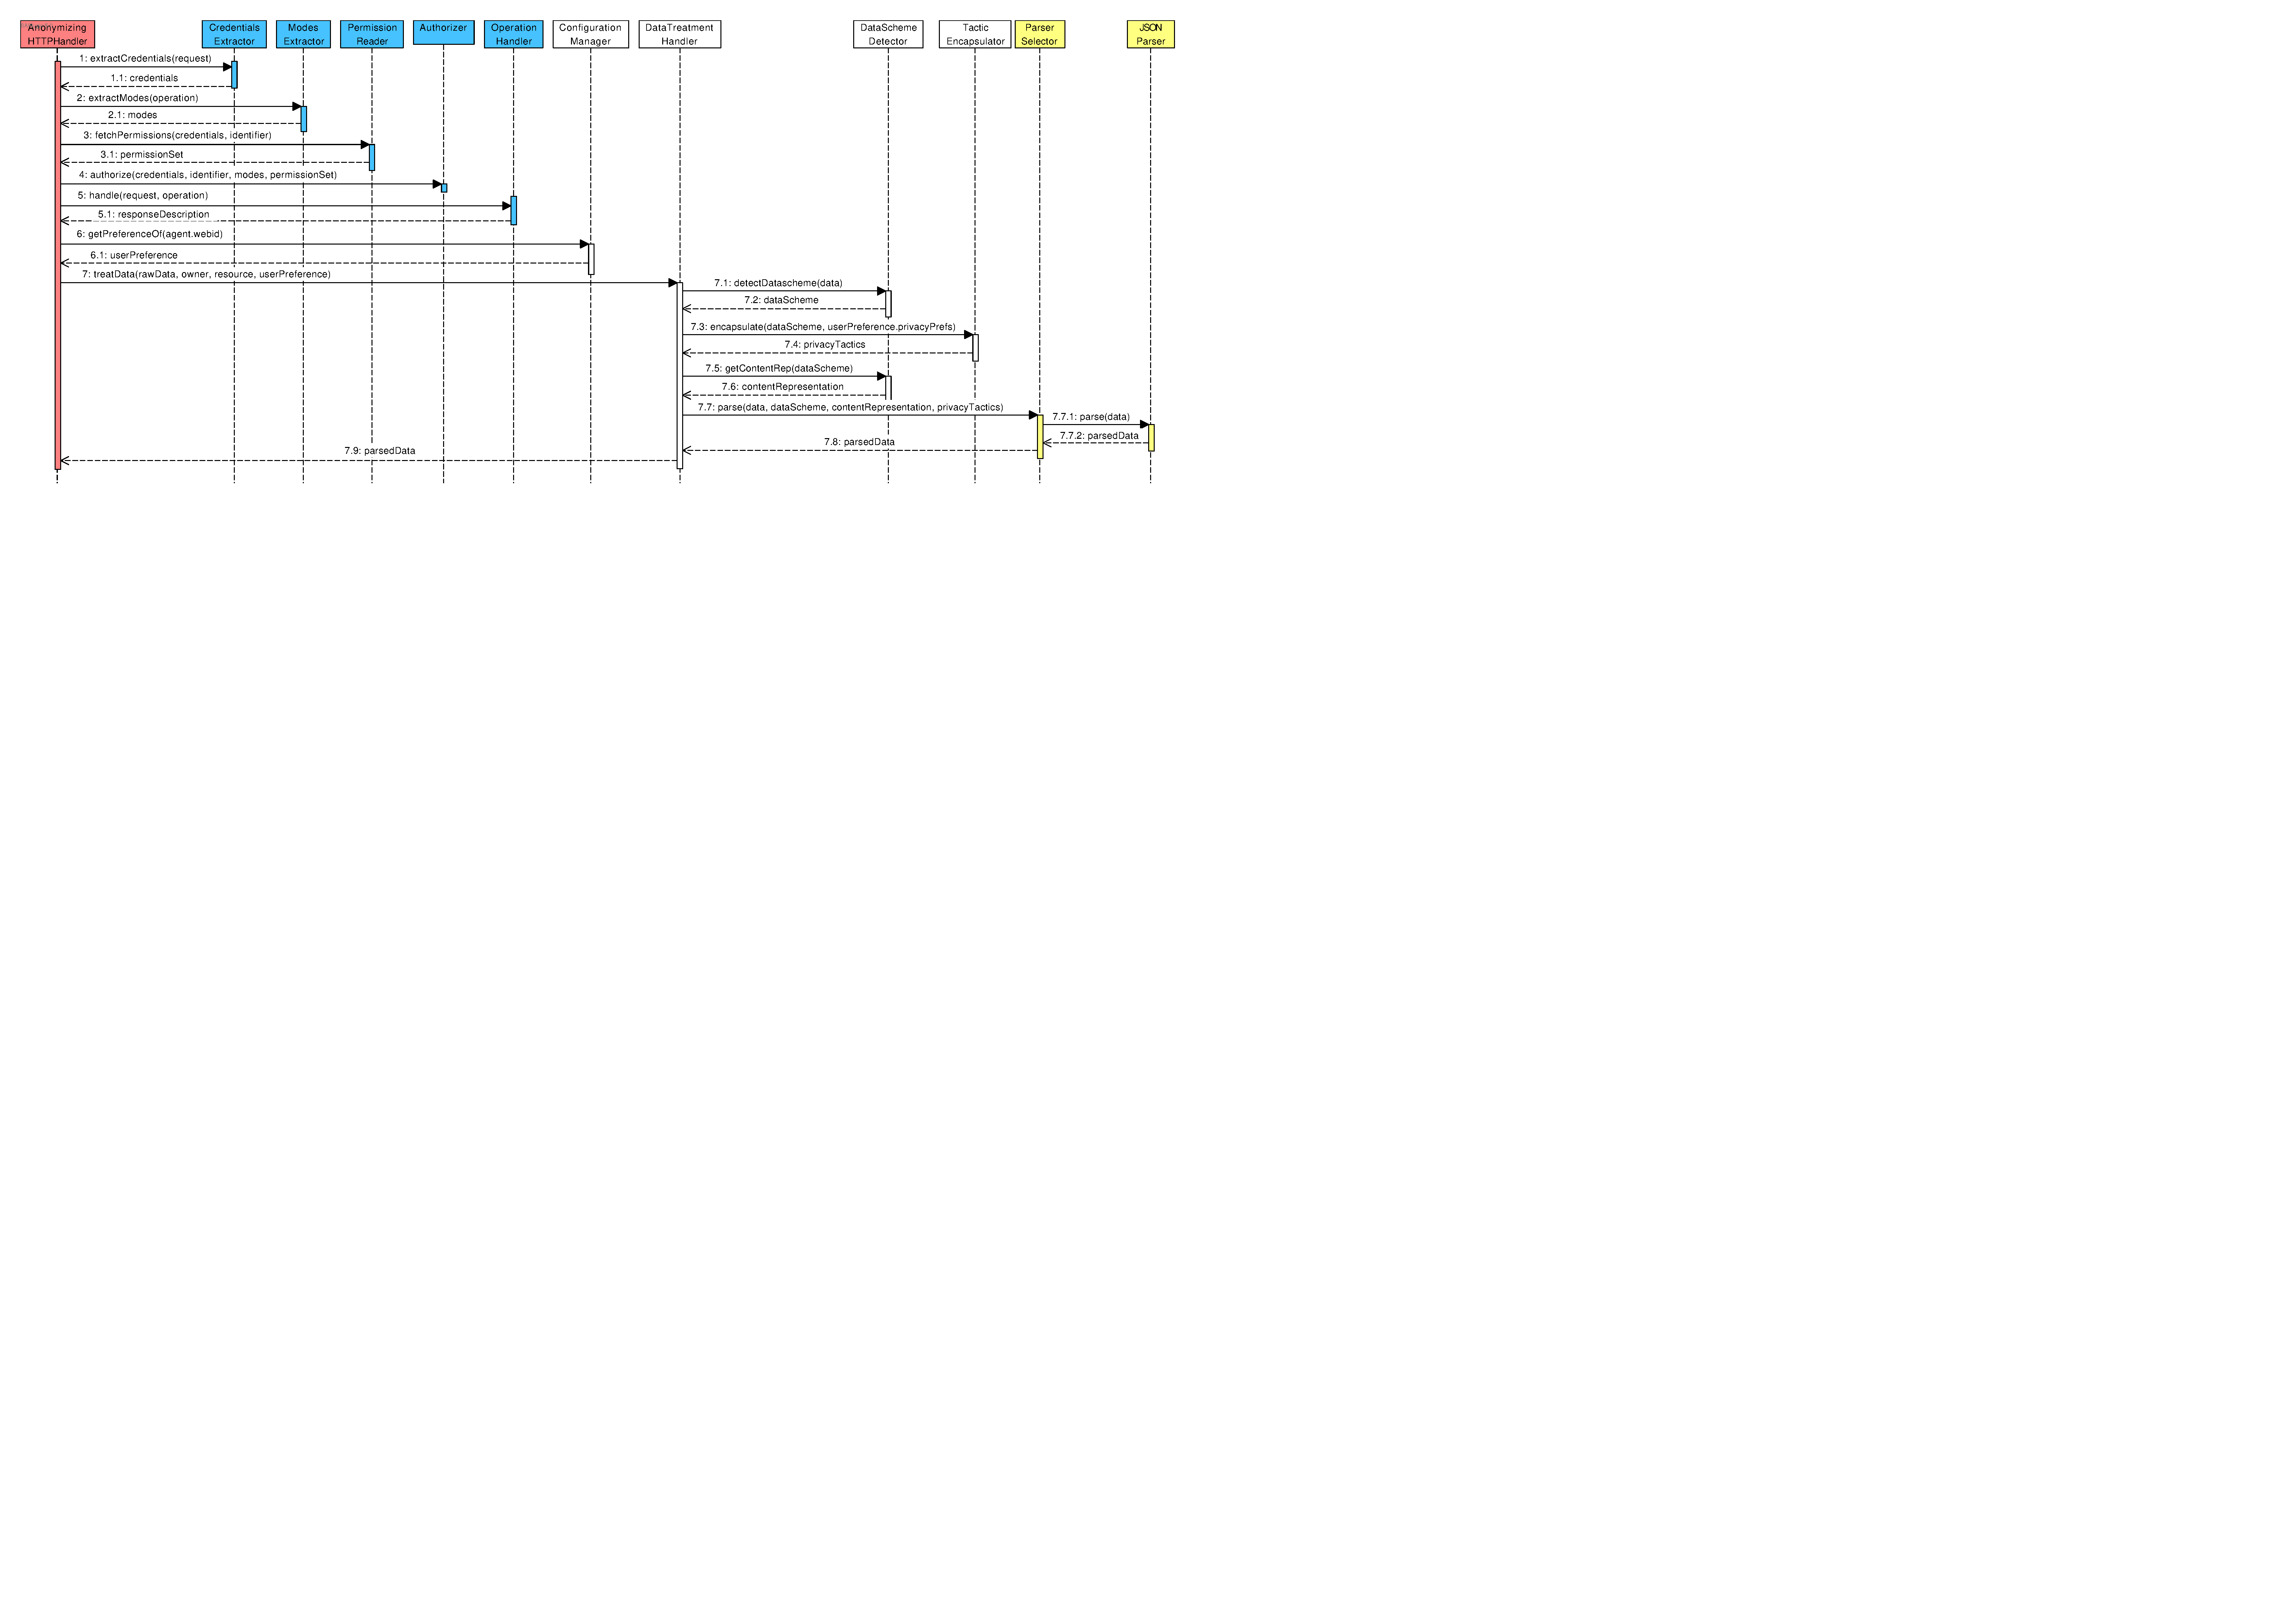
\includegraphics[width=1.0\textwidth]{images/architecture/Rewrite-Flow-PePSA.pdf}
    \caption{Flow of \middleware{} request rewrite}
    \label{fig:pepsa-sequence}
\end{sidewaysfigure}
